\chapter{Foundational Methods}

%% Maybe (Foundational Methods --- supervised)

%%%%%%%%%%%%%%%%%%%%%%%%%%%%%% Regression
\section{Regression}

\textcolor{blue}{Three cases of the {generalized linear model}\index{generalized linear model}, simple, multiple, and polynomial linear regression.}

\textcolor{blue}{TODO: define generalized linear model}

\subsection{Simple Linear Regression}

% C2 of Mastering ML
\textcolor{blue}{Model a \emph{linear} relationship between a response variable and a feature representing an explanatory variable. The relationship is modeled with a linear surface called a hyperplane (A subspace that consists of one dimension less than the dimensionality of the space it occupies e.g. a line in a 2D plot, or a 2D plane in a 3D environment).}

\textcolor{blue}{Simple linear regression consists of two total dimensions (a dimension for the response variable and another for the explanatory) -- the hyperplane, as explained above, has one dimension (line)}

\begin{equation}
{Y \approx \beta_0 + \beta_1 x}
\label{eq:slr_ex}
\end{equation}

\textcolor{blue}{$\approx$ can be read as ``\emph{is approximately modeled as}''. $Y$ is a quantitative response (output/prediction) and $X$ predictor variable(input/feature). $\beta_0$ and $\beta_1$ are two unknown constants representing the intercept and slope, respectively. These unknown values that determine the behavior of the model are known as the model \emph{parameters} or \emph{coefficients}}

\subsubsection{OLS}

\textcolor{blue}{{Ordinary Lease Squares (OLS)}\index{Ordinary Lease Squares (OLS)}, or {Linear Least Squares}\index{Linear Least Squares} is a method for estimating the parameters for a simple linear regression model.}

\textcolor{blue}{Solving OLS for simple linear regression ($y=\beta_0 + \beta_1 x$).}

\textcolor{blue}{First we'll solve for the slope $\beta_1$, where $\beta_1$ is can be found using Eq.\ref{eq:slr_ols_slope}.}

\begin{equation}
{\beta_1 =  \frac{cov(x,y)}{var(x)}}
\label{eq:slr_ols_slope}
\end{equation}

\textcolor{blue}{Variance (Eq.\ref{eq:variance_def}) is the measure of how far the set of values are spread apart -- if all the numbers in a set were equal, their variance would be zero.}

\begin{equation}
{var(x) = \frac{\sum_{i=1}^{n}(x_i - \hat{x})^2}{n-1}}
\label{eq:variance_def}
\end{equation}


\textcolor{blue}{Covariance (Eq.\ref{eq:covariance_def}) is the measure of how much two variable change together -- if two variables increase together, their covariance is positive}

\begin{equation}
{cov(x) = \frac{\sum_{i=1}^{n}(x_i - \hat{x})(y_i - \hat{y})}{n-1}}
\label{eq:covariance_def}
\end{equation}

\textcolor{blue}{After solving for $\beta_1$, $\beta_0$ can be found by rearranging the original equation and \textcolor{red}{substituting in the means of $x$ and $y$}($y=\beta_0 + \beta_1 X$) to become Eq.\ref{eq:slr_ols_intercept}}

\begin{equation}
{\beta_0 =  \bar{y} - \beta_1 \bar{x}}
\label{eq:slr_ols_intercept}
\end{equation}

\subsubsection{Cost}

\textcolor{blue}{Cost or loss function (See \textcolor{red}{local ref?}) is used to define and quantitatively measure the error of the model -- the differences between the predicted and ground truth values. The differences between the training is called the residuals\index{residuals} or training errors where as the differences observed between the test predictions and ground truths are called the prediction or test errors.}

\textcolor{blue}{A common measure of the models fitness may be the {residual sum of squares (RSS)}\index{residual sum of squares (RSS)} (Eq.\ref{eq:rss_def}, where $y_i$ is the observed value and $f(x_i)$ is the predicted value)}

\begin{equation}
{\sum_{i=1}^{n}{(y_i - f(x_i))^2}}
\label{eq:rss_def}
\end{equation}

% see p62 of ISL for more

\subsubsection{Evaluation}

\textcolor{blue}{Several methods exist for measuring the models predictive capability (see \textcolor{red}{local ref?} for more details.)}


\subsection{Multiple Linear Regression}

\textcolor{blue}{Using $n$ predictors:}

\textcolor{blue}{generalization of simple linear regression. Uses multiple features to predict the reponse variable}



\begin{equation}
{Y \approx \beta_0 + \beta_1 X_1 + \beta_2 X_2 + \cdots + \beta_n X_n}
\label{eq:mlr_ex}
\end{equation}


\subsection{Polynomial Regression}

\textcolor{blue}{Special case of multiple linear regression, models a linear relationship between a response variable and polynomial feature terms}

\textcolor{blue}{a linear model that, using polynomial feature terms, can model non-linear relationships.}

\textcolor{blue}{Quadratic regression (second-order polynomial) shown in equation (EQ\ref{eq:quad_regression_def})}

\begin{equation}
{Y \approx \alpha + \beta_1 X + \beta_2 X^2}
\label{eq:quad_regression_def}
\end{equation}










%%%%%%%%%%%%%%%%%%%%%%%%%%%%%% Logistic Regression
\section{Logistic Regression}

\textcolor{blue}{Despite the `regression' bit in the name, logistic regression is a classification model}

\textcolor{blue}{odds ratio\index{odds ratio} (Eq.~\ref{eq:odds_ratio}), where $p$ is representative of the probability of a positive (event we aim to predict) event.}

\begin{equation}
{\frac{p}{1-p}}
\label{eq:odds_ratio}
\end{equation}

\textcolor{blue}{A logit\index{logit} function (Eq.~\ref{eq:logit_def}) is the logarithm of the odds ratio (log-odds)}

\begin{equation}
{logit(p)=\log{\frac{p}{1-p}}}
\label{eq:logit_def}
\end{equation}

\textcolor{blue}{logistic function (sigmoid function) (Eq.~\ref{eq:sigmoid_def}) -- the inverse of a logit function and corresponds to the probability that a certain sample belongs to a particular, positive, class. If the response variable value meats or exceeds the {discrimination threshold}\index{discrimination threshold}, the positive class is predicted.}

\begin{equation}
{S(x)={\frac{1}{1+e^{-x}}}={\frac{e^x}{e^x+1}}}
\label{eq:sigmoid_def}
\end{equation}


%%%%%%%%%%%%%%%%%%%%%%%%%%%%%% KNN
\section{Nearest Neighbors}

\textcolor{blue}{KNN is a lazy learner\index{lazy learner} (a special case of instance-based nonparametric model (see \textcolor{red}{local ref?})): the model memorizes the training dataset rather than learn a discriminative function.}

\textcolor{blue}{The intuition is that instances look alike must be alike.}

\textcolor{blue}{Can be used for classification or regression. To adapt a KNN for regression, the approach is modified to return a prediction of the average target value from the nearest neighbors, rather than the majority label.}

\textcolor{blue}{Due to the curse-of-dimensionality, In practice, nearest neighbors will usually be performed after a dimensionality reduction preprocessing step.}


\subsection{Overview}


% page 188 of FofMLforpred data analytics

\textcolor{blue}{set local models (neighborhoods), where each is defined by a subset of the training data (in nearest neighbors, this is a single instance).}

\textcolor{blue}{A global prediction model based on the full dataset creates a decision boundary between regions of the features space which designates the \textcolor{red}{label?(term)}}

\subsubsection{Distance metric}

\textcolor{blue}{There are four basic requirements for the distance metric:}

\begin{itemize}
	\item Non-negativity: the value must be greater or equal to 0
	\item Identity: if the distance metric between $a$ and $b$ is zero, the two values must be at the same location
	\item Symmetry: the distance metric from $a$ to $b$ must be the same as the distance metric from $b$ to $a$
	\item Triangular inequality: metric($a$,$b$) $\le$ metric($a$,$c$) $+$ metric($b$,$c$)
\end{itemize}

\textcolor{blue}{When calculating the nearest neighbors the terms \textit{distance} and \textit{similarity} may be used interchangeably -- it is important to keep in mind that though they are the ``same'', they are different terms in that the lowest value for distance is ``best'' and the highest value for similarity is ``best''.}

\textcolor{blue}{The default distance metric is the Euclidean distance}

\textcolor{blue}{both the Euclidean and Manhattan distances are special cases of the Minkowski distance}

% see p184 of FofMLforpred data analytics
\textcolor{green}{TODO: more about the Minkowski distance def here}

\textcolor{blue}{Minkowski-based Euclidean distance -- a straight line between two points (Eq~\ref{eq:euclidean_distance_def})}

\begin{equation}
{\sqrt{\sum_{i=1}^{m}{{(a[i] - b[i])}^2}}}
\label{eq:euclidean_distance_def}
\end{equation}

\textcolor{blue}{Manhattan distance (Eq.~\ref{eq:manhattan_distance_def}) -- may also be called the taxi-cab distance, since it is similar to how a driver would have to drive from one point to another on a grid based road system like Manhattan.}

\begin{equation}
{\sum_{i=1}^{m}{abs(a[i] - b[i])}}
\label{eq:manhattan_distance_def}
\end{equation}

\textcolor{blue}{When implementing a nearest neighbor using Euclidean distance, the feature space is partitioned into {Voronoi tessellation}\index{Voronoi tessellation}. New points are assigned to a {Voronoi region}\index{Voronoi region}.}

% see p214 of FofMLforpred data analytics
\textcolor{green}{TODO: More about other similarity measures}

\subsection{K-Nearest Neighbors}

\textcolor{blue}{Since the nearest neighbor algorithm relies on local models, each defined by a single training instance, it is quite sensitive to noise. To address this issue, rather than rely on a single instance, a \textcolor{red}{label} is calculated from a set of $k$ nearest neighbors}

\textcolor{blue}{KNN classification involves i) choosing the number of $k$ (nearest neighbors) and a distance metric, ii) finding the $k$ nearest neighbors, and iii) assigning a class label by majority vote.}

\textcolor{blue}{The optimal value for $k$ will greatly influence the bias-variance trade-off. If the value is too low, there exists a risk of the algorithm being too sensitive to noise and overfitting, where as if the value of $k$ is too high, there is the possibility that a true pattern will be lost.}

\subsection{Considering Imbalanced Data}

\textcolor{blue}{If dealing with imbalanced data, as $k$ increases, the majority label will dominate the feature space.}

\subsubsection{Weighted K-Nearest Neighbors}



\subsubsection{Distance Weighted K-Nearest Neighbors}

\textcolor{blue}{The weight of each instance is a function of the inverse distance to the instance from the specified location. An easy way to implement this is to calculate the reciprocal of the squared distance (Eq.~\ref{eq:weighted_dist_knn}), where $n$ is the neighbor and $m$ is the specified location}

\begin{equation}
{\frac{1}{{dist(m,n)}^2}}
\label{eq:weighted_dist_knn}
\end{equation}

\textcolor{blue}{When calculating weight of each instance, $k$ is set to be a large value and may even be equal to the number of instances in the training set so that all training instances are included in the prediction process.}

\textcolor{blue}{Votes from neighbors that are close to the specified location are assigned a high weight, while distant neighbors are assigned a lower weight value.}

\subsection{Considerations}

% see page 225 of Understanding Machine Learning

\subsubsection{Memory}

\subsection{Other Variations}

% see p196 of FofMLforpred data analytics for more information
\textcolor{blue}{k-d tree, k-dimmensional tree -- balanced binary tree}

\textcolor{blue}{R-Trees}

\textcolor{blue}{B-Trees}

\textcolor{blue}{M-Trees}

\textcolor{blue}{VoRTrees}

%%%%%%%%%%%%%%%%%%%%%%%%%%%%%% Support Vector Machines
\section{Support Vector Machines (SVM)}

\textcolor{blue}{Support Vector Machine (SVM)\index{Support Vector Machine (SVM)}. In order to minimize misclassification errors, the optimization objective is to maximize the margin (distance between the decision boundary (separating hyperplane) and the nearest training samples. These margins are called support vectors). Maximizing the margins, in theory, tend to have lower generalization error, where smaller margins may be more prone to overfitting.}

\textcolor{blue}{(Slack parameter?)}

\textcolor{blue}{Variable can be used to control the width of the margin and help tune the bias-variance trade-off.}

\textcolor{green}{TODO: figure showing difference in width of margins}

\subsection{Kernel SVM}

\textcolor{blue}{kernelized to solve nonlinear classification problems}

\subsubsection{The `Kernel Trick'}

\textcolor{green}{TODO: paras about the kernel trick}

\textcolor{blue}{Transform the training data onto a higher dimensional feature space}

%%%%%%%%%%%%%%%%%%%%%%%%%%%%%% Naive Bayes
%%%%%%%%%%%%%%%%%%%%%%%%%%%%%% Naive Bayes
\section{Naive Bayes}

\textcolor{blue}{typically performs well on small datasets. Compared to logistic regression it is more biased.}

\subsection{Bayes' Theorem}

\textcolor{blue}{Bayes' theorem is a formula (Eq.\ref{eq:bayes_def}) that is used for calculating the probability of an event using prior knowledge and related conditions.}

\begin{equation}
{P(A|B)=\frac{P(B|A)P(A)}{P(B)}}
\label{eq:bayes_def}
\end{equation}

\begin{equation}
{P(y|x_1,\dots,x_n)=\frac{P(x_1,\dots,x_n|y)P(y)}{P(x_1,\dots,x_n)}}
\label{eq:bayes_exp_def}
\end{equation}

% see p131(119) of Mastering ML with SKL
\textcolor{green}{TODO: more...}

% see p131(119) of Mastering ML with SKL
\textcolor{blue}{Variants: multinomial, Gaussian, and Bernoulli.}

\textcolor{blue}{The model is considered Naive because it assumes that all the features are conditionally independent given the response variable.}

\textcolor{blue}{NB assumes all training instances are {independent and identically distributed (i.i.d)}\index{independent and identically distributed (i.i.d)} -- training instances must be independent from each other and drawn from the same probability distribution.}

%%%%%%%%%%%%%%%%%%%%%%%%%%%%%% Decision Trees
%%%%%%%%%%%%%%%%%%%%%%%%%%%%%% Decision Trees
\section{Decision Trees}

\textcolor{blue}{\textcolor{green}{(TODO: revise this para!)} Decision trees make classification decisions based on a series of questions that separate the data into subsets. These questions are chained and result in a tree of questions/decisions where the leaves are considered pure i.e. they contain samples that belong to the same class.}

\textcolor{blue}{Minimum Description Length (MDL) - describes how ``deep'' the tree is allowed to grow.}

\textcolor{blue}{Importance of pruning -- Decision trees can be very deep and can easily lead to overfitting. To help prevent this situation, a limit is set for the maximal depth of a tree. }

\textcolor{blue}{The main advantage to using decision trees is that they are easily interpretable and may often resemble a program developed by hand.}

\subsection{Criterion -- Maximizing Information Gain}

\textcolor{blue}{Term - Information gain -- difference between the impurity of the parent node and the sum of the child node impurities -- the lower the impurity of the child nodes compared to the parent node, the higher the information gain}

\textcolor{blue}{Three commonly used splitting criteria used in binary decision trees: (i) Gini Impurity, (ii) entropy, and (iii) classification error}

\subsubsection{Gini Impurity}

\subsubsection{Entropy}

\subsubsection{Classification Error}

\subsubsection{ID3 Algorithm}

\textcolor{blue}{ID3 or ``Iterative Dichotomizer 3''}


\textcolor{blue}{top-down, recursive, depth-first partitioning of the dataset.}

\textcolor{blue}{Assumes categorical features without any missing values.}

\textcolor{red}{Can be extended to handle continuous descriptive features and continuous target features}

\subsubsection{C4.5 Algorithm}

\textcolor{blue}{Variant of the {ID3 algorithm}\index{ID3 algorithm} that can handle continuous categorical descriptive features and missing features}

\textcolor{red}{uses post-pruning}

\textcolor{blue}{{J48}\index{J48} is an open source implementation of the C4.5 algorithm}

\subsubsection{CART Algorithm}

\textcolor{blue}{The CART algorithm is another variant of the ID3 algorithm.}

\textcolor{blue}{Uses the Gini index}

\textcolor{blue}{Can handle continuous target features}

\subsection{Pruning}

\textcolor{blue}{Can help address overfitting. Pruning is an attempt to reduce the size of the tree while still maintaining a similar empirical error.}

\subsubsection{Pre-pruning}

\subsubsection{Post-pruning}

\section{Random Forests}

% see Breiman, 2001
\textcolor{blue}{Ensemble method. Combine various decision trees, where some may be weak learners\index{weak learner} (\textcolor{green}{def}) and some may be strong learners\index{strong learner} (\textcolor{green}{def}). The final classification will be determined by majority vote from the number of trees.}






\chapter{Artificial Neural Networks}

\textcolor{blue}{If a perceptron is analogous to a single neuron, an artificial neural network (either feedforward or feedback) would be analogous to a brain.}

\r{powerful and general framework for representing non-linear mappings (function approximation) from input features to outputs, where the form of the mapping is controlled by adjustable parameters (weights and biases). Determining the values for these parameters is the ``learning'' or training.}

%%%%%%%%%%%%%%%%%%%%%%%%%%%%%% perceptron
\section{Perceptron}

\r{TODO: overview}

\r{Obligatory Biology figure}

\subsection{History}

\r{McCullock and Pitts -- nerve cell as a simple logic gate with binary outputs.  Where multiple input signals are accumulated and if they exceed a certain threshold an output signal is generated}

\r{$x_i$ represent the input (maybe raw features or output from previous neurons), weights $w_i$ represetn the strengths of the interconnections (analygous to synapses) between the neurons, and the bias $w_0$ represent the threshold for a neuron to be activated.}

\r{Frank Rosenblatt at Cornell Aeonautical Laboratory in late 1950s -- motivated by efforts to simulate the human brain -- the perceptron: an algorithm that would learn the optimal weight coefficients to the input features in order to determine whether an output signal should be produced. The early activation function \textcolor{red}{See more in local ref?} was a simple unit step function.}

\r{Adaline (\textbf{ADA}ptive \textbf{LI}near \textbf{NE}uron) \r{(TODO: WIdrow and Hoff (1960))} -- rather than the weights being updated based on a unit step function like the perceptron, the weights are updated based on a linear activation function. A continuous output value (rather than discrete) is used to compute the model error and update the weights.}

\r{Linear activation function is used for weight updates but a unit step function can still be used to predict the class labels.\textcolor{red}{TODO: figure showing this}}

\subsection{Overview}

\r{advantage: perceptrons are capable of online learning --- the models parameters can be updated on a single training instance rather than a batch of instances}

\r{Though not used too frequently in practice, the perceptron is a building block that later sections in this chapter on artificial neural networks are built upon.}

\r{activation (pre-act(weight $\times$ input - linear transform))}


\begin{figure}[htp]
	\centering
	\includegraphics[width=0.5\textwidth]{example-image-a}\hfil
	\caption{\TD{TODO: diagram of decision space -- 3D change in ``riff'' position. bias - change in position -- model leads to arbitrary complex decision space}}
	\label{fig:ann_decision_space}
\end{figure}

\subsection{Activation Function Basics}

\textcolor{blue}{Basic activation function (Eq.\ref{eq:act_func_basic_def}) where $w$ represents the model's parameters and $b$ represents a bias terms and $act$ is representative of the activation function.}

\begin{equation}
{y = act (\sum_{i=1}^{n}(w_i x_i + b)}
\label{eq:act_func_basic_def}
\end{equation}

\textcolor{blue}{There are many different types of activation functions that may be used. A more in-depth discussion on activation functions is discussed in \textcolor{red}{local ref?}}

\textcolor{blue}{The linear combination of parameters and inputs may sometimes be referred to as the preactivation}

\textcolor{blue}{Rosenblatt's original activation function is the {Heaviside step function}\index{Heaviside step function} ({unit step function}\index{unit step function}), show in Eq.\ref{eq:heaviside_step_func}] \textcolor{green}{TODO: figure}}

\begin{equation}
{out(x) = \left\{
	\begin{array}{ll}
	1 & \quad $when $ x \geq 0 \\
	0 & \quad x < 0
	\end{array}
	\right.}
\label{eq:heaviside_step_func}
\end{equation}

% see p164[152] of Mastering ML w/SKL *para*


\subsection{Limitations}

\textcolor{blue}{}

\textcolor{blue}{nonlinear activation function is necessary to break linearity since computing a series of weighted sums is equivalent to computing a single weighted sum}

\r{around the 1960s --- shown that they could solve a number of problems readily, while unable to solve other problems (that superfically appeared to be a similar level of difficulty). \TD{Perceptrons (book), Minsky and Papert 1969}}

\r{can only classify data sets by a linear hyperplane. However, it is possible to solve linearly inseparable data, provided the data can first be preprocessed. The difficulty lies in the fact that the (pre)processing elemetns are fixed in advance and cannot adapt.}

\subsection{Extending to model linearly inseparable data}

\subsubsection{Kernelization}

\textcolor{blue}{projecting linearly inseparable data into a higher dimensional space (with the intent to make the data linearly separable)}

\subsubsection{Directed Graph}

\textcolor{blue}{Artificial neural network (discussed next, in \textcolor{red}{local ref?}) is a universal function approximator make of a directed graph of perceptrons}

\subsection{Notes}

\textcolor{blue}{If the activation function is a logistic sigmoid activation function, the model is the same as logistic regression.  The difference, however, is that the perceptron can be trained with an online, error driven, approach}

%%%%%%%%%%%%%%%%%%%%%%%%%%%%%% overview
\section{Artificial Neural Networks (ANN)}

\textcolor{blue}{Principals and basic feed forward networks}

\r{The most computationally expensive component is calculating the gradient of the loss function with respect to the parameters of the network}

% see page 233 of Understanding Machine Learning
\r{Artificial neural networks are {universal approximators}\index{universal approximators} -- \textcolor{red}{expand}}

\r{universal approximation theorem \textcolor{green}{(Hornik 1989, Cybenko, 1989)}. Regardless of the function that is attempted to being learned, a large MLP will be able to \textbf{represent} this function. However, it is not guaranteed that the large MLP, despite being a universal \textcolor{red}{approximator} capable of representing the function, is able to \textit{learn} the function}


\subsection{Multi-layer Perceptron}

\r{surprisingly/dangerously robust to bugs}

\r{Not a single multi-layer perceptron with multiple layers, rather it is a network composed of multiple layers of perceptrons. Multi-layer perceptrons, through use of sucessive transformations (multipel layers of adaptive weights) address some of the limitations presented with a single layer perceptron \TD{local ref}.  MLPs, even composed of just two layers, are capable of approximating any continuous functional mapping --- the restriction being that the network must be feed-forward (described in \TD{local ref}) ensuring the outouts are possible to calcualted from as explicit functions of the inputs.}

\r{universal approximator\cite{hornik1991approximation}}

\r{justification for deeper networks --- can be exponentially more compact.}

\subsection{Architecture}

\r{{input layer}\index{input layer}, {hidden layer}\index{hidden layer}, {output layer}\index{output layer}}

\r{the input layer is not counted in the number of layers in a network}

\begin{figure}[htp]
	\centering
	\includegraphics[width=0.5\textwidth]{example-image-a}\hfil
	\caption{\TD{TODO: diagram of neural network showing layers}}
	\label{fig:foundations_ann_overview}
\end{figure}


\subsection{Components}

\begin{figure}[htp]
	\centering
	\includegraphics[width=0.5\textwidth]{example-image-a}\hfil
	\caption{\TD{TODO: labeled diagram of nodes (weights and biases), connections, activation functions}}
	\label{fig:foundations_ann_overview}
\end{figure}


\subsubsection{Nodes / units}

\paragraph{Initialization}

\TD{TODO: initialization methods and for different layers}


\subsubsection{Activation Function}

\TD{TODO: I think this is where I'll talk about activation functions}

%% need for non-linearity
\r{If all the activation functions in the hidden layers of the network were to be linear then it is possible to create a equivalent network without the hidden units. This is due to the principle that the composition of successive linear transformations is itself a linear transformation \TD{show + detail more clearly}. \textcolor{red}{the activation functions of the hidden and output layers may be different.}}

\TD{TODO: step function to sigmoid function -- smoothed version of the step function -- can understand how an input changes the output.}

\r{When considering networks only consisting of threshold activations, we run into the {credit assignment}~\index{credit assignment problem} during training. That is we have no way of determining which of the hidden units is more/less responsible for the incorrect output.  A solution to this issue is to use differentiable activation functions, this then allows for the activation of the output to become differentiable functions of both the input variables and the parameters (weights and biases).}

%% TODO: placement
\r{A sigmoidal hidden unit can be used to approximate a hidden linear unit by scaling the input parameters (weights and biases) to be very small such that the values are small and lie on the linear part of the sigmoidal curve near the origin. Similarly a step function may be approximated by scaling the input parameters (weights and biases) to be very large such that the values are either in the activated or not activated state. Nearly any continuous functional mapping can be represetned by a network consisting of two layers of sigmoidal hidden units.  A network consisting of three or more sigmoidal hidden units can approximate any smooth mapping \TD{Lapedes and Farber 1988}}

\TD{local ref to a more in depth discussion of activation functions.}

%% this likely doesn't belong here
\begin{figure}[htp]
	\centering
	\includegraphics[width=0.3\textwidth]{example-image-a}\hfil
	\includegraphics[width=0.3\textwidth]{example-image-b}\hfil
	\includegraphics[width=0.3\textwidth]{example-image-c}\hfil
	\caption{\TD{TODO: three images of possible decision boundaries created by NN with threshold act.fn and 1,2, and 3 layers. one is a single linear hyperplane, 2 is a non convex and 3 is a disjoint}}
	\label{fig:foundations_ann_layers_decision_region}
\end{figure}

\r{networks having three or more layers of weights can create non-convex and disjoint decision regions. \TD{see Huang and Lippmann 1988 for examples of 2 layers.}. Networks with two layers are not capable of creating arbitrary decision boundries \TD{Gibson and Cownan 1990, Blum and Li, 1991} (also see \TD{fig ref}). However, if the activation function is converted to a sigmoidal activation, it is possible to arbitrarily closely approximate an given decision boundry.}

%%%%%%%%%%%%%%%%%%

\textcolor{blue}{Activation functions are XXXXXXXX}

\subsubsection{Why Non-linear}

\textcolor{blue}{Non-linear is necessary XXXXXXXXXX}

\subsubsection{Advancements}

\textcolor{green}{TODO: From step function to ?selu}

\subsubsection{Popular Activation Functions}

\r{Activation functions can be grouped into two main categories -- smooth and not smooth. Smooth activation functions (such as sigmoid) are differentiable at every point along the function where as the other activation functions are not differentiable at every location (relu).}

% history
%differentiable everywhere, monotonic, and smooth.


\r{linear (see above), }

\textcolor{blue}{ReLu, better because \textcolor{red}{help prevent saturation}, but still have problems \textcolor{red}{can "die" at 0.} }

\textcolor{blue}{ELU fuctions. they prevent the "dying" problem by being \textcolor{red}{non-zero} but their main drawback is that they are more computationally expensive due to the calculation of the exponent.}

\paragraph{Smooth Non-linear}

\subparagraph{Sigmoid}

\textcolor{blue}{The sigmoid\index{sigmoid} activation function.}

\textcolor{blue}{calibrated probability estimate}


% {{{act_smooth_sigmoid}}}
\begin{figure}
	\centering
	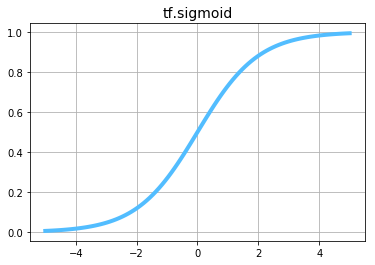
\includegraphics[width=0.65\textwidth]{./sync_imgs/act/smooth/sigmoid.png}
	\label{fig:act_smooth_sigmoid}
\end{figure}

% {{{act_smooth_tangent}}}
\begin{figure}
	\centering
	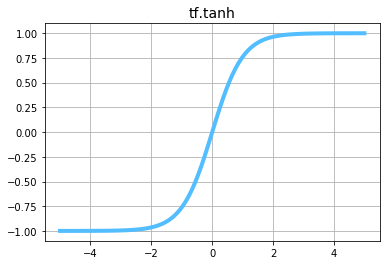
\includegraphics[width=0.65\textwidth]{./sync_imgs/act/smooth/tangent.png}
	\label{fig:act_smooth_tangent}
\end{figure}

\subparagraph{ELU}

\textcolor{blue}{\textcolor{red}{CITE}. Smooth, monotonic, and non-zero in the negative portion of the input. The main drawback is that they are more computationally expensive (due to calculating the exponential)}


\begin{equation}
{
	ELU = f(x) = \left\{
	\begin{array}{ll}
	\alpha(e^x - 1) x & \quad $for$ \ x < 0 \\
	x & \quad $for$ \ x \ge 0
	\end{array}
	\right.
}
\label{eq:act_elu_def}
\end{equation}


% {{{act_smooth_elu}}}
\begin{figure}
	\centering
	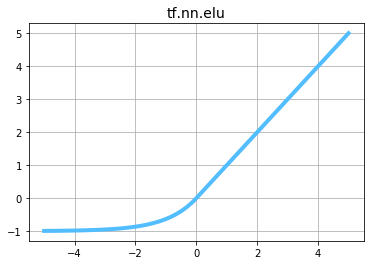
\includegraphics[width=0.65\textwidth]{./sync_imgs/act/smooth/elu.png}
	\label{fig:act_smooth_elu}
\end{figure}

% {{{act_smooth_selu}}}
\begin{figure}
	\centering
	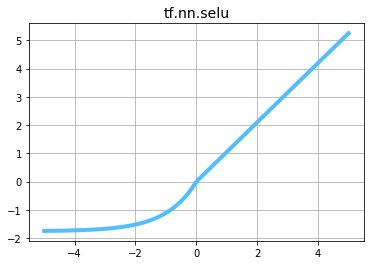
\includegraphics[width=0.65\textwidth]{./sync_imgs/act/smooth/selu.png}
	\label{fig:act_smooth_selu}
\end{figure}


\subparagraph{Softplus}

\textcolor{blue}{continuous and differentiable at zero. However, due to the natural log and exponential function, there is added computation compared to th ReLU.}

% typcially discouraged in practice since ReLU achieves similar results and is less computationally expensive

\begin{equation}
{
	Softplus = f(x) = \ln{(1+e^x)}
}
\label{eq:act_softplus_def}
\end{equation}


% {{{act_smooth_softplus}}}
\begin{figure}
	\centering
	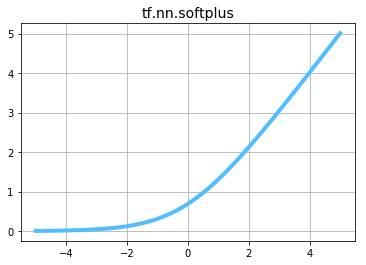
\includegraphics[width=0.65\textwidth]{./sync_imgs/act/smooth/softplus.png}
	\label{fig:act_smooth_softplus}
\end{figure}

% {{{act_smooth_softsign}}}
\begin{figure}
	\centering
	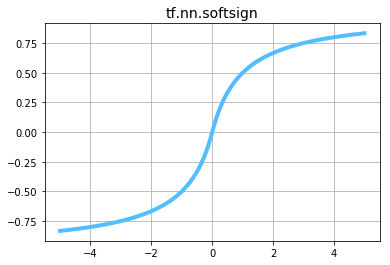
\includegraphics[width=0.65\textwidth]{./sync_imgs/act/smooth/softsign.png}
	\label{fig:act_smooth_softsign}
\end{figure}


\paragraph{Not Smooth Non-linear}

\subparagraph{ReLU}

\begin{equation}
{
	ReLU = f(x) = \left\{
	\begin{array}{ll}
	0 & \quad $for$ \ x < 0 \\
	x & \quad $for$ \ x \ge 0
	\end{array}
	\right.
}
\label{eq:act_relu_def}
\end{equation}

% {{{act_notsmooth_relu}}}
\begin{figure}
	\centering
	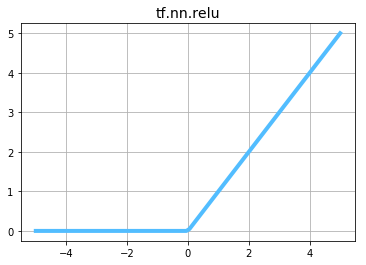
\includegraphics[width=0.65\textwidth]{./sync_imgs/act/notsmooth/relu.png}
	\label{fig:act_notsmooth_relu}
\end{figure}

\subparagraph{Leaky ReLU}

\textcolor{blue}{The Leaky ReLU (Eq~\ref{eq:act_leaky_relu_def}) was designed in attempt to address the dying ReLU issue \textcolor{red}{CITE}. Rather than simply outputting a zero in the negative range, the Leaky ReLU will will have a small non-zero slope (user specified) -- allowing weight updating and training to continue.}

\textcolor{green}{TODO: randomized Leaky ReLU \textcolor{red}{cite} --- $\alpha$ (from PReLU) is sampled from a uniform distribution randomly. The net-effect could be considered similar to drop out since, technically, there is a different network for each value of $\alpha$, resulting in an ensemble of sorts. At test time, the values for $\alpha$ are averaged.}

\begin{equ}[!ht]
	\begin{equation}
	{
		Leaky ReLU = f(x) = \left\{
		\begin{array}{ll}
		N x & \quad $for$ \ x < 0 \\
		x & \quad $for$ \ x \ge 0
		\end{array}
		\right.
	}
	\label{eq:act_leaky_relu_def}
	\end{equation}
	\caption{where $N$ is a constant. $N$ is typically set to 0.01}
\end{equ}

% {{{act_notsmooth_leakyrelu}}}
\begin{figure}
	\centering
	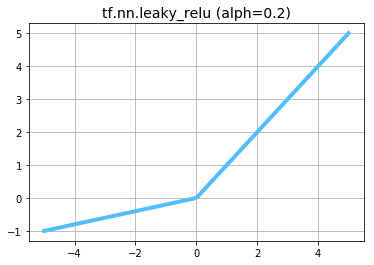
\includegraphics[width=0.65\textwidth]{./sync_imgs/act/notsmooth/leakyrelu.png}
	\label{fig:act_notsmooth_leakyrelu}
\end{figure}

\subparagraph{ReLU6}

\textcolor{blue}{In general, this function is referred to as a {ReLUN}\index{ReLUN} function, where $N$ is some constant. However, in practice, $6$, was determined to be the optimal value.\textcolor{red}{CITE}. \textcolor{red}{This capped value, may help learn the sparse values sooner.} By having the upper limit bounded, the prepare the network for a fixed point precision for inference --- if the upper limit is unbounded, then you may loose too many bits to \textcolor{red}{Q} portion of the fixed point number.}


\textcolor{blue}{Similar to the ReLU fuction, only the output is capped to six in the positive domain.}

\begin{equation}
{
	ReLU6 = f(x) = min{(max{(0,x)},6)}
}
\label{eq:act_ReLU6_def}
\end{equation}

% {{{act_notsmooth_relu6}}}
\begin{figure}
	\centering
	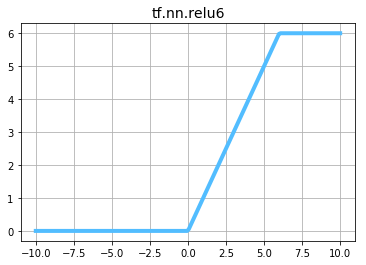
\includegraphics[width=0.65\textwidth]{./sync_imgs/act/notsmooth/relu6.png}
	\label{fig:act_notsmooth_relu6}
\end{figure}

\subparagraph{PReLU}

\begin{equ}[!ht]
	\begin{equation}
	{
		PReLU = f(x) = \left\{
		\begin{array}{ll}
		\alpha x & \quad $for$ \ x < 0 \\
		x & \quad $for$ \ x \ge 0
		\end{array}
		\right.
	}
	\label{eq:act_prelu_def}
	\end{equation}
	\caption{where $\alpha$ is a parameterized --- a learned parameter from training.}
\end{equ}

\r{Parametric Rectified Linear Unit (PReLU) \cite{he2015delving}}

\textcolor{blue}{$\alpha$, rather than being hard coded, is determined during training by the data. The logic being that the value would be more optimal than we could set \textcolor{red}{CITE}}

% {{{act_notsmooth_prelu}}}
\begin{figure}
	\centering
	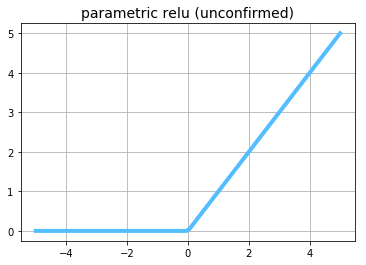
\includegraphics[width=0.65\textwidth]{./sync_imgs/act/notsmooth/prelu.png}
	\label{fig:act_notsmooth_prelu}
\end{figure}







%%%%%%%%%%%%%%%%


\subsection{Characterization}

\subsubsection{Types: Feed-forward vs Feedback}

\textcolor{blue}{Feed-forward --- Directed acyclic graph of artificial neurons. Feedback contain feedback connections that are fed back into itself. When feedforward are include these feedback connections, they become considered recurrent neural networks.}

\paragraph{Feed-forward}

\r{``general framework for representing non-linear functional mappings between a set of input variables and a set of output variables''}

\subparagraph{Layered networks}

\begin{figure}[htp]
	\centering
	\includegraphics[width=0.5\textwidth]{example-image-a}\hfil
	\caption{\TD{TODO: layered network diagram}}
	\label{fig:foundations_ann_layered_network}
\end{figure}

\r{Whereas a single layer network is composed of linear combination of input variables, that are then, transformed by a non-linear activation function, more general functions are creating layered networks that are composed of successive layers of processing units (adaptive weights) with connections running from every unit in one layer to every unit in the next.}

\subparagraph{General topologies}

\begin{figure}[htp]
	\centering
	\includegraphics[width=0.5\textwidth]{example-image-b}\hfil
	\caption{\TD{TODO: general topology}}
	\label{fig:foundations_ann_general_topology}
\end{figure}

\r{general topologies}

\paragraph{Feedback}

\subsubsection{Terminology}

\r{Considered \textit{networks} since they are typically composed of many different functions --- creating a ``network''.}

\r{Considered \textit{neural} since they are \textbf{loosely} inspired by neuroscience.}

\r{layer --- a layer may be considered a group of units that act in parallel. The layer will extract representations from the input, that are (in theory) more useful to the specific task.  Chaining together these layers results in a form of progressive \IDI{data distillation}.}

\r{Visible and Hidden Layers. Visible layers are called visible since they contain variables that are ``visible'', where as the hidden layers extract increasingly abstract features -- hidden since their values are not given in the raw data, but rather an output from a previous layer.}



\subsection{Learning: Backpropagation}

% see p196[184] of Mastering ML w/SKL
\TD{TODO: whoooo, this is going to be a big one. understand how each component contributes to the error and adjust accordingly.}

\r{popularized by \TD{Rumelhard, Hinton and Williams (1986)}, but similar ideas were discussed earlier by \TD{Werbos 1974}, and \TD{Parker 1985}}

\r{error backpropagation is used for evaluating the dervivatives of an error function with respect to the parameters (weights and biases) of the network}

\r{Iterative algorithm consisting of two main components --- the forward, then reverse, pass.}

% see p.141(156) - 146(161) of NNbishop
\TD{MORE}

\TD{Example}

\paragraph{Forward pass}

\r{In the forward pass inputs are propagated through the network and derivatives of the error functuion, with respect to the parameters (weights and biases) are evaluated. Propagation o ferrors through the network, calculating the derivatives, can be applied to may different error functions.}

\r{it becomes important to use a computationally efficient method for evaluating these derivatives \TD{local ref}}

\r{During this stage is when the errors are propagated through the network.}

\paragraph{Backward pass}

\r{In the Backward pass, the previously calcuated derivatives are used to compute the adjustments to the parameters --- propagated in reverse through the network (from cost function to input layer) and each node is updated -- \TD{TODO: expand}.}

\r{Many optimization schemes \TD{local ref} may be used to adjust the parameters by using the calculated derivatives from the forward pass.}

\r{The calculated derivatives are used by the majority of training algorithms}

%% p116 of neural networks, p131 on tablet
\TD{Hessian matrix is a matrix containing the second derivative of a function. The second derivative provides information about the curvature of the function.}

% see p197-201[180] of Mastering ML w/SKL
\TD{TODO: figure showing sample calculation}


% See p207 of DL

\r{also sometimes called \IDI{reverse-mode differentiation}.  Calculate the contribution that each parameter had on the loss value}

\r{\IDI{symbolic differentiation} --- compute a gradient function for the chain (chain rule) mapping parameter values to gradient values}

\subsubsection{Back-propagation efficiency}

%% see para in p146(161) of bishop NN

\subsubsection{Chain Rule}

\r{See \textcolor{red}{local ref to math prereq section}}

\TD{TODO: chain rule}

\r{Backpropagation is typically used with an optimization algorithm (see \textcolor{red}{local ref?})}

\subsection{Multi-layer perceptrons}

% TODO: this doesn't really belong here.. will need ot work on placement

\subsection{Operations}

\subsection{Convolution}
% TODO: I'm not sure how I'm going to structure these yet or where I'll be placing them

% TODO: https://arxiv.org/abs/1904.11486
% https://www.youtube.com/watch?v=HjewNBZz00w


\r{really when we refer to the convolution opperation, we are lying and actually refering to the cross-correlation, since we don't rotate the kernel 180$\deg$.}


% Graham Taylor
\r{weighted averaging operation in time or space}

\r{translational invariant --- if a feature is learned in one corner, it can be observed in another area as well.}

\r{translation equivariant --- }

\r{DNN on an image may not take advantage of the ``stationarity'' (statistics) of an image. Patterns don't depend on the spatial location.}

\r{spatial hierarchies --- \TD{TODO: figure raw data, abstract edges+, then more distinct images, then closer output to the output, then the final label}}

\textcolor{red}{local ref to TensorFlow implementation}

\r{typcially a feature extraction phase (consisting of convolutional and pooling layers) followed by a classifier block (dense layers).}

%%%% popular layer types
\textcolor{green}{TODO: feature maps, (height, width, and depth (also called channels axis)). Stride, filter size, depth. talk about parameters}

\r{The output feature map (every dimension in the depth axis is a feature/filter) --- after a convolution operation the depth of a layer is no longer representative of a color channel (like RGB), it is now representative of a feature extracted by the convolutional operation, these are called filters.}

\TD{Strided Convolution\cite{springenberg2014striving}}

\TD{Dilated Convolution --- `atrous' convolution. (famously used by wavenet), which is convenient in time series analysis.}

\r{weight tieing}


\textcolor{green}{TODO: figure}

\begin{figure}[htp]
	\centering
	\includegraphics[width=0.5\textwidth]{example-image-a}\hfil
	\caption{Figure example of convolution operation on 2d image \textcolor{green}{TODO}}
	\label{fig:conv_2d_example_calc}
\end{figure}

\begin{figure}[htp]
	\centering
	\includegraphics[width=0.5\textwidth]{example-image-b}\hfil
	\caption{Figure example of convolution operation on 3d image \textcolor{green}{TODO}}
	\label{fig:conv_2d_depth_example_calc}
\end{figure}

\textcolor{green}{TODO: examples of how different filter values and strides can effect the output dimensions.}




\subsection{Pooling}
% TODO: I'm not sure how I'm going to structure these yet or where I'll be placing them -- pooling really does not belong under feed forward

\TD{TODO: examples of max vs average pooling}

%%%%%% research
\textcolor{blue}{Pooling may not fully determine learned deformation stability -- possibly filter smoothness\cite{ruderman2018learned}}

\r{downsampling}

\r{Why? importance of reducing the number of params.}

\TD{L2-pooling}

\TD{L2-pooling over the features or channels.}

\TD{additional --- learned/parameterized pooling}

\begin{figure}[htp]
	\centering
	\includegraphics[width=0.5\textwidth]{example-image-a}\hfil
	\caption{Figure example of max pooling operation on 2d image \textcolor{green}{TODO: I want this figure to be basic 2d}}
	\label{fig:pooling_max_2d_ex_a}
\end{figure}

\begin{figure}[htp]
	\centering
	\includegraphics[width=0.5\textwidth]{example-image-b}\hfil
	\caption{Figure example of average pooling operation on 3d image \textcolor{green}{TODO: I want this figure to be 3d}}
	\label{fig:pooling_avg_3d_ex_a}
\end{figure}


\r{may be better to use convolutional layers in place of the pooling layers\cite{springenberg2014striving}}

%%%%%%%%%%%%%%%%%%%%%%%%%%%%%% feedforward
\section{Feed-forward}

\textcolor{blue}{A feedforward network can be represented as a directed acyclic graph -- a directed graph in which there exist no cycles in the underlying graph, with nodes representing neurons and connected by edges}

\textcolor{blue}{layer depths ~ to hierarchy of features}




%%%% popular layer types

\textcolor{blue}{convolution}

\textcolor{blue}{capsule}


%%%%%%%%%%%%%%%%%%%%%%%%%%%%%% feedback
\section{Feedback or Recurrent}

\textcolor{green}{TODO: Overview}

%%%% popular layer types

\textcolor{blue}{LSTM}

\textcolor{blue}{GRU}

\r{RNNs or ``\textit{\textbf{r}}ecurrent \textit{\textbf{n}}eural \textit{\textbf{n}}etworks'' are used for a variety of purposes but are typically designed with sequences of data as an input in mind. They are similarin concept to a standard/feed-forward netowrk, with the major distinction being that they also have connections that point ``backwards'' i.e. they have connections that feed into themselves.}

\r{Are capable fo working on sequences of arbitrary lengths, rather than fixed-sized inputs}

\subsection{Foundation}

\r{An example of an RNN diagram is shown in \TD{fig}. However, this representation is misleading since it does not show ``every'' connection in the model --- most notably, the recurrent connections.  RNNs may also be often represented in diagrams as ``unrolled'' (\TD{fig}). The unrolled RNN is easier to visualize how these recurrent connections are included.  This makes it easier to understand how each timestep is dependent on not only the current input (at the particular time step), but also dependent on ``all'' previous time steps. It is often stated that at a certain timestep (n), the output has ``memory'' since it is a function of all the previous time steps.}


\footnotetext{the term ``all'' is emphasized here since it is the goal to include information from all previous time steps. This is true in theory, however, this is not always the case in practice. This is discussed further in \ALR{}}

\subsection{Simple RNN and Recurrent Neuron}

\TD{Diagram of the inside of a RNN neuron}


\subparagraph{Overview}

\TD{todo}


\section{Common Problems}

Two well known main problems with RNNs.

\begin{enumerate}[noitemsep,topsep=0pt]
	\item Maintaining states are expensive
	\item Vanishing and/or exploding gradients
\end{enumerate}

\TD{hardware acceleration}

\subsection{Maintaining States}


\subsection{Addressing Vanishing and Exploding Gradients}

\r{Propagating signals through a long/deep network without loosing (vanishing gradient) or overamplifying the signal (exploding gradient) is difficult.  There have been a few advances to address this issue.}

\begin{enumerate}[noitemsep,topsep=0pt]
	\item Architecture (different cell types, memory schemes)
	\item Initialization Strategies
	\item Activation Function
\end{enumerate}




\section{Architecture}

\TD{a different section focusing on this}



\subsection{Cell Advancements}

\subsubsection{LSTM}

Introduced in 1997 %\cite{hochreiter1997long}

\r{detect long term dependencies in sequence}

\r{two state vectors, short and long term}

\r{Main motivation: learning what to store in the long-term state and what to ``forget''.}

\r{at each time step, some information is ``stored'' and some information is ``forgotten''.}

\paragraph{Fully Connected Layers}


\begin{enumerate}[noitemsep,topsep=0pt]
	\item Main
	\item \textit{Gate Controllers}
	\begin{enumerate}[noitemsep,topsep=0pt]
		\item Forget
		\item Input
		\item Output
	\end{enumerate}
\end{enumerate}

\r{The gate controllers use a logistic activation fuction (output a range from 0 to 1). This output is then fed through an element-wise multiplication function and thus if the value is $0$, the gate is ``closed'', and $1$ if the gate is ``open''.}

\r{These gates are able to potentially:}

\begin{enumerate}[noitemsep,topsep=0pt]
	\item Recognize an important input
	\item Store the important input in a long-term state ()
	\item Preserve the information for as long as it's needed
	\item Extract the important information when needed
\end{enumerate}


\subparagraph{Main}

\begin{figure}
	\centering
	\includegraphics[width=0.5\textwidth]{example-image-a}\hfil
	\caption{\TD{Main Layer DIAGRAM}}
	%\label{}
\end{figure}

\r{This allows for the same basic functionality as a ``standard'' RNN cell --- however, the output, rather than being only sent to the next cell, is now partially stored in the long-term state.}


\subparagraph{Forget}

\r{Determines which part of the long-term state is forgotten/erased.}

\begin{figure}
	\centering
	\includegraphics[width=0.5\textwidth]{example-image-a}\hfil
	\caption{\TD{Forget Layer DIAGRAM}}
	%\label{}
\end{figure}



\subparagraph{Input}

\r{Determines which part of the output from the \textbf{main layer} are kept in the long-term state.}

\begin{figure}
	\centering
	\includegraphics[width=0.5\textwidth]{example-image-a}\hfil
	\caption{\TD{Input Layer DIAGRAM}}
	%\label{}
\end{figure}

\subparagraph{Output}

\r{Determines which part of the long term state is ``relevant'' (read and output).}

\begin{figure}
	\centering
	\includegraphics[width=0.5\textwidth]{example-image-a}\hfil
	\caption{\TD{Output Layer DIAGRAM}}
	%\label{}
\end{figure}


\paragraph{Other}

\subparagraph{Peephole Connections}

\r{In basic LSTM cells, the gate controller can only look at the input and previous short-term state. Peephole connections, proposed in 2000 \TD{cite gers2000recurrent} add an extra connection that allows for the gate controller to also see information from the long term state as well. }

\r{The previous long-term state also becomes an input to the forget and input gate. The current long-term state becomes an intput to the output gate.}



\subsubsection{GRU}

\r{The GRU (gated recurrent unit) is a varient of the LSTM cell \TD{cite - cho2014learning}. The main modifications include:}

\begin{itemize}[noitemsep,topsep=0pt]
	\item Both state vectors are merged into one state vector
	\item A single gate controller determines the \textbf{Forget} and \textbf{Input} gate
	\begin{itemize}[noitemsep,topsep=0pt]
		\item If the gate output is a 1, the input is open and the forget gate is closed. If the gate output is 0, the input gate is closed and the forget gate is open
	\end{itemize}
	\item \r{The output gate is removed and a new controller exists that controls which part of ht previous state will be ``shown'' to the main layer}. At each timestep the full state vector is output.
\end{itemize}



\subsection{Initialization}

\subsection{Activation Functions}

\subsection{Notes -- add}

\r{A recent paper \TD{greff2017lstm}, comares three LSTM variants and makes three main observations:}

\begin{itemize}[noitemsep,topsep=0pt]
	\item no significant architecture improvements over LSTMs
	\item forget gate and the output activation function are the most critical components
	\item \TD{hyperparams...}
\end{itemize}












\chapter{Common Operations}

\chapter{Overview}

% TODO: this chapter needs serious restructuring/organization consideration

\section{Introduction}

\textcolor{green}{TODO: Tensorflow is an open-source library for numerical computation (not only as a deep/machine learning framework), released by google XXXXXXXXX.}

\textcolor{green}{TODO: There are many different deep learning frameworks}

\textcolor{green}{TODO: why use a deep learning framework}

\section{High-level Overview of Components}

\textcolor{green}{TODO: paras with local refs to components}

\textcolor{green}{TODO: Diagram of tensorflow at a high level}


\section{TensorFlow Essentials}

\subsection{API Hierarchy}

\subsection{Placeholders, feed\_dict, Variables and Constants}

\textcolor{blue}{using get\_variable to create the variable}

\subsection{Coding Style}

\textcolor{blue}{Imperative vs lazy evaluation.}

\subsection{Graphs}

\textcolor{blue}{TODO: Graphs.}

\textcolor{blue}{directed}

\textcolor{blue}{acyclic}

\textcolor{blue}{Why directed acyclic graph (DAG) representation? Language and Hardware Portability -- Developers get to develop programs in a high level language (like python) and have the TensorFlow execution engine execute (written in C++) the model on different platforms (targeted for exact hardware)}

\subsection{Sessions}

\textcolor{blue}{TODO: Sessions.}

\subsection{Tensors}

\textcolor{blue}{TODO: what is a tensor. Tensor --- an n dimensional array of data. they ``flow" through the (directed, acyclic) graph --- hence, TensorFlow}

\section{Workflow}

\textcolor{green}{TODO: Diagram of a typical workflow}

% lazy evaluation
\textcolor{blue}{first step is to build the graph, the second step is to execute the graph (in a session, which will evaluate to numpy arrays)}

% eager mention
\textcolor{blue}{There exists another mode of operation called ``eager'', in which the operations are executed imperatively (tf.eager is discussed in further detail in \textcolor{red}{local ref})}

\textcolor{blue}{TODO: list of overloaded operations, common arithmetic operators/shorthand}

% TODO: this belongs somewhere else
\textcolor{blue}{Note about how training is more computationally expensive than inference}

\section{Debugging TensorFlow}

\textcolor{blue}{Before writing any TensorFlow, I'd like to share some tips and tools to debug TensorFlow programs.}


\textcolor{blue}{error messages are your friend. Use the error message to isolate and debug the operation that is causing problems.}

\textcolor{blue}{two pieces of information: i) stack trace and ii) error message (type+message and operation) }

\subsection{Common Errors}
% tensor shape
% scalar-vector mismatch
\subsubsection{Shape}

% TODO: show how to use these common operations and their output
\textcolor{blue}{some common operations to change the shape of a tensor may included i) tf.reshape() ii) tf.expand\_dims(), iii) tf.slice(), and iv) tf.squeeze() --- expand and squeeze are inverses} 

\subsubsection{Data Type}
% data type mismatch

\subsection{Debugging Tools}

\subsubsection{tf.Print}
% log specific tensor values
%TODO: Code Examples

\subsubsection{tfdbg}

%TODO: Code Examples

% python super_tf_model.py --debug

\subsubsection{TensorBoard}

%TODO: diagram examples

\textcolor{blue}{Using TensorBoard for monitoring is discussed in a later section(\textcolor{red}{local ref}). The scope in this section will focus on using TensorBoard to debug a program}

\subsubsection{Logging and Verbosity}

% different modes overview debug --> fatal
% info = development, warn = production
% tf.logging.set_verbosity(tf.logging.INFO)







\chapter{Applied Neural Networks}

\chapter{Overview}

% TODO: this chapter needs serious restructuring/organization consideration

\section{Introduction}

\textcolor{green}{TODO: Tensorflow is an open-source library for numerical computation (not only as a deep/machine learning framework), released by google XXXXXXXXX.}

\textcolor{green}{TODO: There are many different deep learning frameworks}

\textcolor{green}{TODO: why use a deep learning framework}

\section{High-level Overview of Components}

\textcolor{green}{TODO: paras with local refs to components}

\textcolor{green}{TODO: Diagram of tensorflow at a high level}


\section{TensorFlow Essentials}

\subsection{API Hierarchy}

\subsection{Placeholders, feed\_dict, Variables and Constants}

\textcolor{blue}{using get\_variable to create the variable}

\subsection{Coding Style}

\textcolor{blue}{Imperative vs lazy evaluation.}

\subsection{Graphs}

\textcolor{blue}{TODO: Graphs.}

\textcolor{blue}{directed}

\textcolor{blue}{acyclic}

\textcolor{blue}{Why directed acyclic graph (DAG) representation? Language and Hardware Portability -- Developers get to develop programs in a high level language (like python) and have the TensorFlow execution engine execute (written in C++) the model on different platforms (targeted for exact hardware)}

\subsection{Sessions}

\textcolor{blue}{TODO: Sessions.}

\subsection{Tensors}

\textcolor{blue}{TODO: what is a tensor. Tensor --- an n dimensional array of data. they ``flow" through the (directed, acyclic) graph --- hence, TensorFlow}

\section{Workflow}

\textcolor{green}{TODO: Diagram of a typical workflow}

% lazy evaluation
\textcolor{blue}{first step is to build the graph, the second step is to execute the graph (in a session, which will evaluate to numpy arrays)}

% eager mention
\textcolor{blue}{There exists another mode of operation called ``eager'', in which the operations are executed imperatively (tf.eager is discussed in further detail in \textcolor{red}{local ref})}

\textcolor{blue}{TODO: list of overloaded operations, common arithmetic operators/shorthand}

% TODO: this belongs somewhere else
\textcolor{blue}{Note about how training is more computationally expensive than inference}

\section{Debugging TensorFlow}

\textcolor{blue}{Before writing any TensorFlow, I'd like to share some tips and tools to debug TensorFlow programs.}


\textcolor{blue}{error messages are your friend. Use the error message to isolate and debug the operation that is causing problems.}

\textcolor{blue}{two pieces of information: i) stack trace and ii) error message (type+message and operation) }

\subsection{Common Errors}
% tensor shape
% scalar-vector mismatch
\subsubsection{Shape}

% TODO: show how to use these common operations and their output
\textcolor{blue}{some common operations to change the shape of a tensor may included i) tf.reshape() ii) tf.expand\_dims(), iii) tf.slice(), and iv) tf.squeeze() --- expand and squeeze are inverses} 

\subsubsection{Data Type}
% data type mismatch

\subsection{Debugging Tools}

\subsubsection{tf.Print}
% log specific tensor values
%TODO: Code Examples

\subsubsection{tfdbg}

%TODO: Code Examples

% python super_tf_model.py --debug

\subsubsection{TensorBoard}

%TODO: diagram examples

\textcolor{blue}{Using TensorBoard for monitoring is discussed in a later section(\textcolor{red}{local ref}). The scope in this section will focus on using TensorBoard to debug a program}

\subsubsection{Logging and Verbosity}

% different modes overview debug --> fatal
% info = development, warn = production
% tf.logging.set_verbosity(tf.logging.INFO)








\chapter{Unsupervised}

\r{The reality is that data is not always labeled.}

\r{unsupervised learning is capable of finding hidden patterns in the underlying structure of hte data.}

\r{attempts to represent data with increaingly fewer parameters}

\textcolor{blue}{Discovering hidden structures or patterns in unlabeled training data.}

\TD{Neighborhood-Based Methods \ref{nearest_neighbors} \r{lazy learners  -- learn how to label new instances based on proximity to existing instances}}

% TODO: placement / may need to rename+restructure sections
\textcolor{blue}{unsupervised methods may be commonly used in two main settings:}
\begin{enumerate}[noitemsep,topsep=0pt]
	\item Data Exploration
	\begin{itemize}[noitemsep,topsep=0pt]
		\item Visualization (clustering \textcolor{red}{local ref})
	\end{itemize}
	\item Preprocessing (e.g. prior to a supervised method): unsupervised pretraining may be considered a form of regularization
	\begin{itemize}[noitemsep,topsep=0pt]
		\item Compressing (dimensionality reduction \textcolor{red}{local ref})
		\item Creating new/different representations
	\end{itemize}
\end{enumerate}

\r{regularization, feature engineering, detecting outliers -- also used for detecting how different new (incoming) training data is from the current distribution.}

\r{popular applications --- anomaly detection, group segmentation, preprocessing (dimensionality reduction)}

\subsection{TODO}

\TD{evaluating unsupervised learning systems are harder to evaluate than supervised learning systems.}

%%%%%%%%%%%%%%%%%%%%%%%%%%%%%% clustering
\section{Clustering}

\textcolor{blue}{Clustering, may be referred to as cluster analysis, involves grouping observations such that instances in the same group (cluster) are more similar to one another than they are to instances from another group --- where ``similarity'' is defined by `some metric'. Clustering may be used to explore a dataset}

\textcolor{blue}{Clustering may be used to perform {image quantization}\index{image quantization}, a lossy compression methods that will replace similar colors with a single color to reduce the size of the image file.}

\r{Finding sub groups where observations are more similar to eachother based on some similarity measure. Clustering is sometimes referred to as ``unsupervised classification'' and is often used to explore a dataset.}

\r{An example of clustering may be to group a collection of documents into categories, or songs into genres. examples --- recommendation system}

\subsection{Common Algorithms}

\r{Major clustering algorithms}
\begin{itemize}[noitemsep,topsep=0pt]
	\item k-means
	\item hierarchical clustering
	\item DBSCAN
\end{itemize}

\subsubsection{K-means}

\r{iterative process -- moves centroid (center of cluster) to mean position of instances then reassigning instances to clusters by closest centroid}

\r{will continue to iterate until some stopping criteria is satisfied.}

\r{To avoid unlucky initialization leading to convergence on local optima, K-means may be repeated many times (dozens to hundreds) with a random initialization. The initialization values that lead to the minimum cost function is then determined to be best.}

\r{$k$ (positive integer less than the number of instances in the training set) specifies the number of clusters/centroids}

\r{minimizes the within-cluster/group variation (also known as the initeria)}

\r{the more clusters, the initeria decreases}

\TD{TODO: k-means cost function}

\r{important to note that K-means will not necessarily converge on the global optimum. Different runs will result in slightly different cluster assignments.}

\r{randomly assigns each observation to one of the k clusters}

\r{reassigns obervations in order to minimize the Euclidean distance between the observation and cluster's center.}

\r{several runs -- lowest total sum of within-cluster variation}

\TD{TODO: variations such as mini-batch k-means}

\r{}

\paragraph{Local Optima}

\textcolor{blue}{unlucky initialization}

\paragraph{Selecting K}

\TD{todo: Overview}

\r{No right/theoretical answer, need to perform trial and error: optimal number found by minimizing the cost function}

\paragraph{Elbow Method}

\textcolor{blue}{The elbow method is used to select the optimal number of clusters if $k$ is not specified by the problems context.}

% rough
\textcolor{blue}{plot of the final cost function value is plotted against the value of $k$. As $k$ increases, the average distortion will decrease as each cluster will have fewer instances and they will be closer to their respective centroid. This decline in dispersion will decline most at a point and then slowly continue to decline -- the point at which the dispersion decreases the most can be considered the elbow (and considered by the elbow method to be the best value for $k$)}

\textcolor{green}{TODO: diagram showing data clusters}

\textcolor{green}{TODO: diagram showing $k$ vs dispersion related to above cluster diagram}



\subsubsection{Hierarchical Clustering}

\TD{overview}

\TD{agglomerative --- tree-based clustering that builds a dendogram --- upside-down tree}

\r{after evaluation, the user can decide which size of tree tey want to use.}

\r{by default Euclidian distance is used, but other similarity metrics can also be used \TD{link to reference}}

\TD{figure example}

% TODO: this likely diens't fit here
\TD{Ward --- Ward's minimum variance method}

\subsubsection{DBSCAN}

\TD{\textbf{D}ensity-\textbf{b}ased \textbf{s}patial \textbf{c}lustering of \textbf{a}pplications with \textbf{n}oise.}

\r{user defined: minimum number of instances and distance}

\r{any instance that is not within a specified distance is labeled as an outlier}

\r{arbitrarily shaped clusters}

\subsubsection{HDBSCAN}

\r{Hierarchical DBSCAN --- groups on density then uses distance measure on the created groups iteratively}


\subsection{Evaluating}

\textcolor{blue}{There are no labels - can still evaluate using intrinsic measures}

\textcolor{blue}{measuring distortion of clusters}

\subsubsection{Silhouette Coefficient}

\textcolor{blue}{The {silhouette coefficient}\index{silhouette coefficient} is a measure of compactness and separation of clusters. The silhoette coefficient is calculated per instance or for a set of instances (where the value is calculated to be the mean of the individual instances in the group). Eq.\ref{eq:silhouette_coef_def} can be used to calculate the silhouette per instance, where $d$ is the mean distance between the instance and the instances in the next closest cluster and $b$ is hte mean distance between the instances in the indicated cluster.}

\begin{equation}
{s = \frac{db}{max(d,b)}}
\label{eq:silhouette_coef_def}
\end{equation}







%%%%%%%%%%%%%%%%%%%%%%%%%%%%%% Dimensionality Reduction
\section{Dimensionality Reduction}
\label{unsupervised_dimensionality_reduction}

\r{Dimensionality reduction is typically used to reduce the dimensions in a feature representation while retaining as much information as possible.}

\r{reproduce the orginal dataset from teh reduced feature set as well as possible.}

\r{Motivation: i) mitigate issues caused by the curse of dimensionality ii) compress data iii) visualize and explore datasets and improve interpretability -- interpreting data in high dimensions is harder than in lower dimension spaces (particularly three or less). May also be used to compress data before being used by another learning algorithm.}

\r{Example --- projecting 3D data into a 2D space.}

\r{project the raw high-dimensuional input data into  a lower-dimensional space by only \TD{iteratively removing the least explainatory dimensions.}}

\TD{Two major branches of dimensionality --- linear and nonlinear (manifold). The difference is in the projection, one is linear and the other is, you guessed it, nonlinear.}

\r{Unsupervised Transformations --- Dimensionality Reduction --- where the goal is to reduce the dimensionality of the data while retaining as much as the relevant information as possible}

%% topic extraction

\r{A high number of features may be computationally costly. Ability to generalize may be reduced if some of the features capture noise or are irrelevant to the underlying relationship. The goal could be to find the features that account for the greatest changes in the response variable}

\subsection{Principal Component Analysis}

\textcolor{green}{{Principal Component Analysis (PCA)}\index{Principal Component Analysis (PCA)} may also be known as the {Karhunen-Love Transform (KLM)}\index{Karhunen-Love Transform (KLM)} }

\textcolor{red}{eigen-decomposition of the covariance matrix}

%p232[220] of Masstering ML w/SKL
\textcolor{red}{``PCA is most useful whe 'the variance of the dataset is distributed unevenly across the dimensions'' }

% TODO: get var/covar defs (currently in regression tex)
\textcolor{blue}{carvariances between each par of dimensions in a dataset are described in a {covarience matrix}\index{covarience matrix} }

\r{combine highly correlated features -- represent with fewer (linearly uncorrelated) features}

\r{searches for linear combinations in all input variables --- retains as much of the variation (salient information) as possible (some is lost)}

\TD{several variants --- incremental PCA, nonlinear (kernel PCA), sparse (sparse PCA)}

\TD{NOTE: it is important to ensure the features are on the same scale before performing PCA.}

\subsubsection{Linear}

\paragraph{Incremental PCA}

\r{small batches.}

\paragraph{Sparse PCA}

\TD{generates PCs slightly differently than normal PCA. Searches for linear combinations in only some of the input variables.}

\subsubsection{Nonlinear}

\paragraph{Kernel PCA}

\TD{more}

\r{similarity funciton (kernel method). Effective when the original feature set is not linear separable}

\TD{type of kernel}

\TD{kernel coefficient (gamma) -- \ALR -- popular radial basis function kernel}


\subsection{Singular value decomposition (SVD)}

\TD{TODO}

\TD{rank matrix}

\subsection{Random Projection}

\TD{TODO}

\textcolor{red}{Johnson-Lindenstrauss lemma}

\r{two versions: standard (gaussian random projection) and sparse (sparse random projection)}

\subsubsection{Gaussian Random Projection}

\r{linear projection}

\subsubsection{Sparse Random Projection}

\TD{TODO}

\section{Nonlinear dimensionality reduction}

%%%% % plus index - unsupervised method
% see p156 of DL for more
\TD{manifold learning (or nonlinear dimensionality reduction)--- {manifold}\index{manifold}, though having a more formal mathematical meaning, will be considered a connected region for our machine learning purposes. --- Nonlinear transormation. PCA and random projection project the data linearly from high to low dimension.}

\subsection{Isomap}

\TD{isomap -- type of manifold learning. estimates the geodesic or curved distance (rather than euclidean) between a point and its neighbors}

\r{relative to neighbors on a manifold \textcolor{red}{rather than a plane?}}

\subsection{Multidimensional Scaling (MDS)}

\TD{TODO}

\subsection{Locally Linear Embedding (LLE)}

\r{segments data into smaller components (neighborhoods), \textcolor{red}{models each component as a linear embedding}}

\r{preserves distance within neighborhoods}

\TD{TODO}

\subsection{t-Distributed Stochastic Neighbor Embedding (t-SNE)}

\TD{TODO}

\TD{t-distributed stochastic neighbor embedding (t-SNE) --- non-linear --- }


\r{two probability distributions, one over pairs of points in a high-dimensional space and another in a low dimensional space. minimizes the \TD{kullback-Leibler divergences} between these two probability distributions.}


\textcolor{red}{nonconvex cost function}

\r{different initializations will generate different results --- no stable solution}

\textcolor{red}{HELLO}

\section{Non-geometric, no distance metric}

\subsection{Dictionary Learning}

\TD{TODO}

\r{learns sparse representation of the original data}

\r{atoms --- vectors in the dictonary. vectors are binary vectors. instances are reconstructed as weighted sum of atoms. easily identify vectors with the most nonzero values}

\r{the dictionary can be undercomplete or overcomplete. undercomplete: atoms $<$ features in the original dataset, or overcomplete: atoms $>$ features in the original dataset.}

\TD{mini-batch version of dictionary learning}


\subsection{Independent Component Analysis (ICA)}

\TD{Separate blended signals into individual components (signal processing)}

\subsection{TODO: others}


% TODO: find a good text on this -- this should be an in depth section
% TODO: dataset for individual voices ina coffeehouse


\TD{Latent Dirichlet allocation}

\r{nonlinear --- multidimensional scaling (MDS), locally linear embedding (LLE), independent componenet analysis (ICA), t-distributed stochastic neighbor embedding (t-SNE), dictionary learning, random trees embedding}

\subsection{Autoencoders}
% TODO: this may not belong here

\TD{discussed more in depth in \ALR}

\r{encoder and decoder --- trained at once}

\r{May be described as a network that learns an approximation of an identity function. reconstructs original features --- hidden layers, reduce parameters (forced to learn salient features), subsequent layers learn increasingly complex relations from the preceeding layers.}

\r{if given too much capacity (``too'' many parameters), the autoencoder may (likely should) simply memorize the observations.}

\paragraph{Undercomplete vs Overcomplete}
\r{undercomplete --- if the constrain encoders output to fewer dimensions than the input}

\r{overcomplete --- when the encoders output dimensions are larger than the input dimensions. typically used in addition to a form of regularization.}

%\paragraph{Sparse vs Dense}



\subsection{Generative Adversarial Networks}
% TODO: this may not belong here

\r{described in more detail in \ref{generative_adversarial_network}}

\subsection{Hidden Markov Model}
% TODO: this may not belong here

\r{simple markov model -- states change stochastically. future states only depend on current state (not prior states)}

\r{Hidden Markov model -- learn propbable next state given what is known about hte sequence of previous states}


% TODO: format / other
%\input{./foundations/unsupervised/applications}


\chapter{Semi-supervised}

\section{Semi-Supervised}

\textcolor{green}{TODO: overview}

\subsection{Examples}

\textcolor{green}{TODO: Examples}


\chapter{Common Architectures}


\TD{Overview}

% TODO: I'm still not sure if I should divide this up by ``types'' of architectures or types of problems and the architectures used to solve them.. maybe both? unsure...


Images and Videos
\begin{itemize}[noitemsep,topsep=0pt]
	\item Classification
	\item Segmentation
	\begin{itemize}[noitemsep,topsep=0pt]
		\item Semantic segmentation (where we don't differentiate between instances)
		\item Instance segmentation
	\end{itemize}
	\item Object detection
\end{itemize}


\subsection{Spatial Data}

\r{types of problems -- spatial to spatial (1:1), spatial to sequence, spatial to value (single or multiple)}

\subsubsection{Convolutional Approaches}

% Survey on CNNs
% TODO: a lot here -- good read
\TD{A Survey of the Recent Architectures of Deep Convolutional Neural Networks \cite{DBLP:journals/corr/abs-1901-06032}}


\subsubsection{Image Classification}
% Graham Taylor talk
\r{alexnet, network-in-network, inception/google lenet (end with $1 \times 1 \times N_{classes}$ into a global average pooling layer), vggnet}

\r{Resnet (similar to highway networks) --- skip connections ``residual modual/block'' (dynamically adjusting depth) (others in this time: fractal nets, stochastic XXXX nets, where skip connections are shortcut paths)}

\r{DenseNet --- where these skip connections are taken to an extreme. also, concatenation, not summation}

\r{Squeeze and Excitation network --- adaptive recalibration of feature maps. \TD{TODO}}

% fit into an architecture ``timeline''
\TD{ResNeXt\cite{xie2017aggregated}}


\subsection{Object Detection}

\r{sliding window and use each window as input to a classifier. But the problem is that we need to apply the classifier to a huge number of locations and scales and aspect ratios. A potential solution to this problem is to use region proposals.}

\r{region proposals were introduced by R-CNN \TD{cite}, where conventional methods were used to propose regions for the CNN to classify. It's important to note that most regions are not square may need to be warped to be insert to the CNN}

\r{Bbox regression is also used --- how much to offset the region proposal.}


\r{fast R-CNN proposed regions by using the feature maps from a layer from a CNN that was previously trained (VGG or Resnet, for example). after identifying the regions, then crop-resize, then CNN over each region, then get output (class + bbox regression.)}

\r{faster r-cnn. Insert a region proposal network (RPN) to predict proposals from features --- in this architecture, there are actually four losses to jointly train 1) object/net RPN, 2) box/net RPN, 3) Class prediction, and 4) final bounding box score.}


\subsection{Segmentation}

\r{fully convolution --- dowsample to upsample: 1) efficency when using convs on smaller dimensional inputs 2) latent representation}

\r{CNN and RPN --- nice results \TD{cite}}

\r{mask R-CNN --- also used for pose prediction}

% code: https://github.com/facebookresearch/detectron2/tree/master/projects/PointRend
% blog: https://ai.facebook.com/blog/using-a-classical-rendering-technique-to-push-state-of-the-art-for-image-segmentation/
\TD{PointRend: Image Segmentation as Rendering \cite{Kirillov2019PointRendIS}}


\section{Text: Natural Language Processing}


\section{Structured data: Tablular}


\section{Other Common Architectures}




% chapter: model compression
\chapter{Model ``Compression''}

% this section will likely be moved around
motivation

\begin{itemize}[noitemsep,topsep=0pt]
	\item Model (output) performance
	\begin{itemize}[noitemsep,topsep=0pt]
		\item regularization (through reduction of number of parameters)
	\end{itemize}
	\item Model performance
	\begin{itemize}[noitemsep,topsep=0pt]
		\item memory/storage --- by creating physically smaller networks
		\item energy --- computation, latency, which supports edge depolyments
	\end{itemize}
\end{itemize}

\section{Quantization}


\r{reduces the precision of parameters in a model}

\r{latency, memory}

\r{some fixed-point accellerators become available in edge settings}

\subsection{When}

\subsubsection{during training}

\subsubsection{post-training}

\r{calibration data}

\section{Weight Pruning}

%TODO: https://github.com/he-y/Awesome-Pruning -- repo of recent pruning work

% intial skeleton influence by:
\TD{The initial structure and citations were heavily influenced by \cite{lange2020_lottery_ticket_hypothesis}}

\TD{SNIP: Single-shot Network Pruning based on Connection Sensitivity \cite{DBLP:journals/corr/abs-1810-02340}}

\r{reduces the overall number of parameters}

\r{in practice, this often refers to setting the parameters of a particular ``node'' to zero and making it untrainable during training.}

\TD{Comparing Rewinding and Fine-tuning in Neural Network Pruning \cite{Renda2020ComparingRA} --- Learning rate rewinding}

\TD{Deconstructing Lottery Tickets: Zero \cite{DBLP:journals/corr/abs-1905-01067} --- SuperMasks}

\TD{The Early Phase of Neural Network Training \cite{Frankle2020TheEP}}

% `` identify highly sparse trainable subnetworks at initialization, without ever training, or indeed without ever looking at the data''
\TD{Synaptic Flow Pruning (SynFlow) --- Pruning neural networks without any data by iteratively conserving synaptic flow \cite{Tanaka2020PruningNN}}

% code: https://github.com/varungohil/Generalizing-Lottery-Tickets
\TD{One ticket to win them all: generalizing lottery ticket initializations across datasets and optimizers \cite{Morcos2019OneTT}}


\subsubsection{What to remove}



\paragraph{relationship of nodes to nodes pruned}

\subparagraph{unstructured}

\r{no consideration for relationship between pruned weights}

\subparagraph{structured}

\r{prunes ``groups'' of weights.}

\paragraph{relationship of nodes to architecture}

\subparagraph{local}

\r{enforcment of a percent of weights pruned at each layer}

\subparagraph{global}

\r{total percent of weights are pruned, no restriction layer wise.}

\subsubsection{Deciding what to remove}

\r{common thought: large magnitude parameters are ``more important'' and thus should be removed less --- which is counterintuitive to concepts such as l2 regularization which penalize large magnitude parameters.}

\TD{other techniques}

\subsubsection{When to prune}

\begin{itemize}[noitemsep,topsep=0pt]
	\item Before training
	\item During training
	\item After training
\end{itemize}

\subsubsection{Pruning mechanism}

\begin{itemize}[noitemsep,topsep=0pt]
	\item One shot (prune all at once)
	\item Iterative
\end{itemize}

\section{Topology}

\r{more efficient model topology}

\subsection{Distillation}

\subsection{Tensor Decomposition}
% Not sure what this is -- from coursera


% TODO: this fits somewhere in this chapter, but not necessarily `here'
\subsection{The Lottery Ticket Hypothesis}


\TD{Original paper --- The Lottery Ticket Hypothesis: Training Pruned Neural Networks \cite{DBLP:journals/corr/abs-1803-03635} --- iterative pruning. Dense network at initialization contains a number of ``winning tickets''}


\TD{Stabilizing the Lottery Ticket Hypothesis \cite{DBLP:journals/corr/abs-1903-01611}}

\TD{IMP with rewind}

% CODE: https://github.com/RICE-EIC/Early-Bird-Tickets
\TD{Drawing early-bird tickets: Towards more efficient training of deep networks \cite{You2020DrawingET}}

\TD{Playing the lottery with rewards and multiple languages: lottery tickets in RL and NLP \cite{Yu2020PlayingTL}}



% chapter: training dynamics
\chapter{Training Dynamics}

% TODO: I'm not sure where this section fits yet

\TD{Critical Learning Periods in Deep Neural Networks \cite{DBLP:journals/corr/abs-1711-08856}}

\TD{Characterizing Structural Regularities of Labeled Data in Overparameterized Models\cite{jiang2020exploring}}

\TD{Do deep neural networks learn shallow learnable examples first? \cite{mangalam2019deep}}


\chapter{Adversarial Machine Learning}
%TODO: I'm not convinced this is the right location for this section

\TD{survey \TD{Adversarial Attacks and Defences: {A \cite{DBLP:journals/corr/abs-1810-00069}}}}

\TD{a bit cat and mouse}

% TODO: common attacks and defences

% TODO: robustness

\r{Adversarial Machine Learning, or adversarial ML, is .....}


\r{sometimes refered to as ``optical illusions'' for AI}


\r{adversarial input or ``adversarial example'' as first refered to as by \TD{Intriguing properties of neural networks \cite{Szegedy2014IntriguingPO}}}

\TD{follow up to original \TD{Explaining and Harnessing Adversarial Examples \cite{Goodfellow2015ExplainingAH}}}

\r{other extreme, labeling human unrecognizable images confidently \TD{Deep Neural Networks are Easily Fooled: High Confidence Predictions for Unrecognizable Images \cite{DBLP:journals/corr/NguyenYC14}}}

\TD{\cite{papernot2018deep}}

\TD{Towards Evaluating the Robustness of Neural Networks \cite{DBLP:journals/corr/CarliniW16a}}

\TD{Towards Deep Learning Models Resistant to Adversarial Attacks \cite{Madry2018TowardsDL}}

\section{Attacks}

\TD{section on attacks}

\TD{single pixel attack}

\section{Defenses}

\TD{section on defenses}

\r{possible first \TD{Towards Deep Neural Network Architectures Robust to Adversarial Examples \cite{Gu2015TowardsDN}}}

\section{Implications}

\TD{section on implications}
